
\newcommand{\chapterpepperapp}{Kapitel 4. }
\chapter{Konzept: Pepper App für die Hochschule}
\label{sec:anwendungsfall-hochschule}
\lhead{\chapterpepperapp \emph{Konzeptionierung: Pepper App für die Hochschule}}

\section{Die Vorüberlegungen}
Nachdem wir uns darauf geeinigt haben, einen Anwendungsfall für den Roboter Pepper zu entwickeln und sich dieser auf den Alltag an der Hochschule Bremerhaven beziehen soll, haben wir uns damit konfrontiert gesehen, uns Gedanken darüber zu machen, wie genau eine Interaktion zwischen einem Studenten oder einer Lehrkraft und dem Roboter stattfinden kann. Aufgrund der aktuellen Beschlüssen der Regierung, ist das Leben auf dem Campus fast zum Stillstand gekommen, wodurch sich für Pepper wenig Einsatzgebiete ergeben. Wir gehen jedoch davon aus, zu einer neuen Normalität zurück zu gelangen, und werden Pepper dahingehend vorbereiten.

Folgende Fragen sind für uns zentral:
\begin{itemize}
    \item Wie sieht der Alltag auf dem Campus aus?
    \item Wann soll Pepper mit wem interagieren?
    \item Welche Funktionalitäten wollen wir implementieren?
    \item Wo setzen wir welche Werkzeuge ein?
    \item Wo fangen wir an?
\end{itemize}

Wir sind dann ziemlich schnell darauf gekommen, dass wir eine klare Struktur benötigen, um unsere Aufgaben und Ziele klar zu definieren. Daraufhin ist folgende Skizze entstanden, welche grob die Hauptfunktionalitäten unseres Projektes festhält:
\begin{figure}[H]
    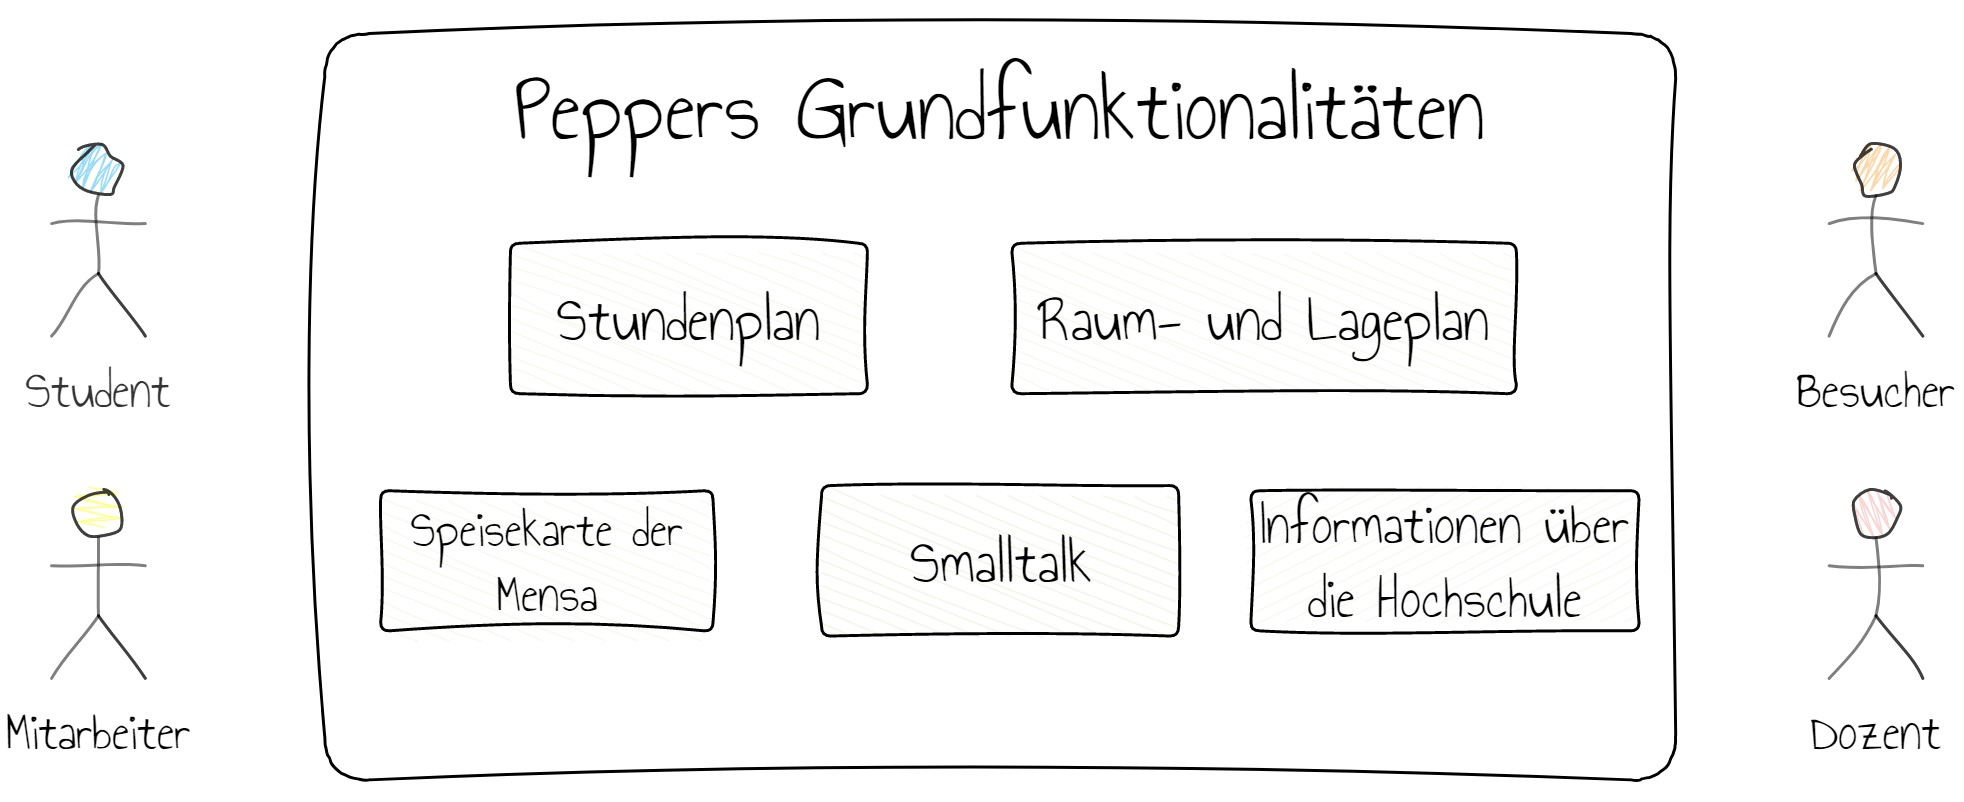
\includegraphics[width=\textwidth]{Figures/pepper-usecase-skizze.jpg}
    \caption{Skizze: Konzeptplanng der Anwendungsfälle}
    \label{fig:integration}
    \centering
\end{figure}


% Nachfolgend sind unsere vordefinierten Grundfunktionalitäten zu aufgelistet.

% \begin{itemize}
%     \item Stundenplan
%     \item Raum- und Lageplan
%     \item Speisekarte der Mensa
%     \item Smalltalk
%     \item Informationen über die Hochschule
% \end{itemize}

Auf Grundlage der diese Grundfunktionalitäten haben wir damit begonnen die Anwendungsfälle weiter zu spezifizieren in dem wir diese in einem Anwendungsfall-Diagramm zusammen getragen haben. \\

\begin{figure}[H]
    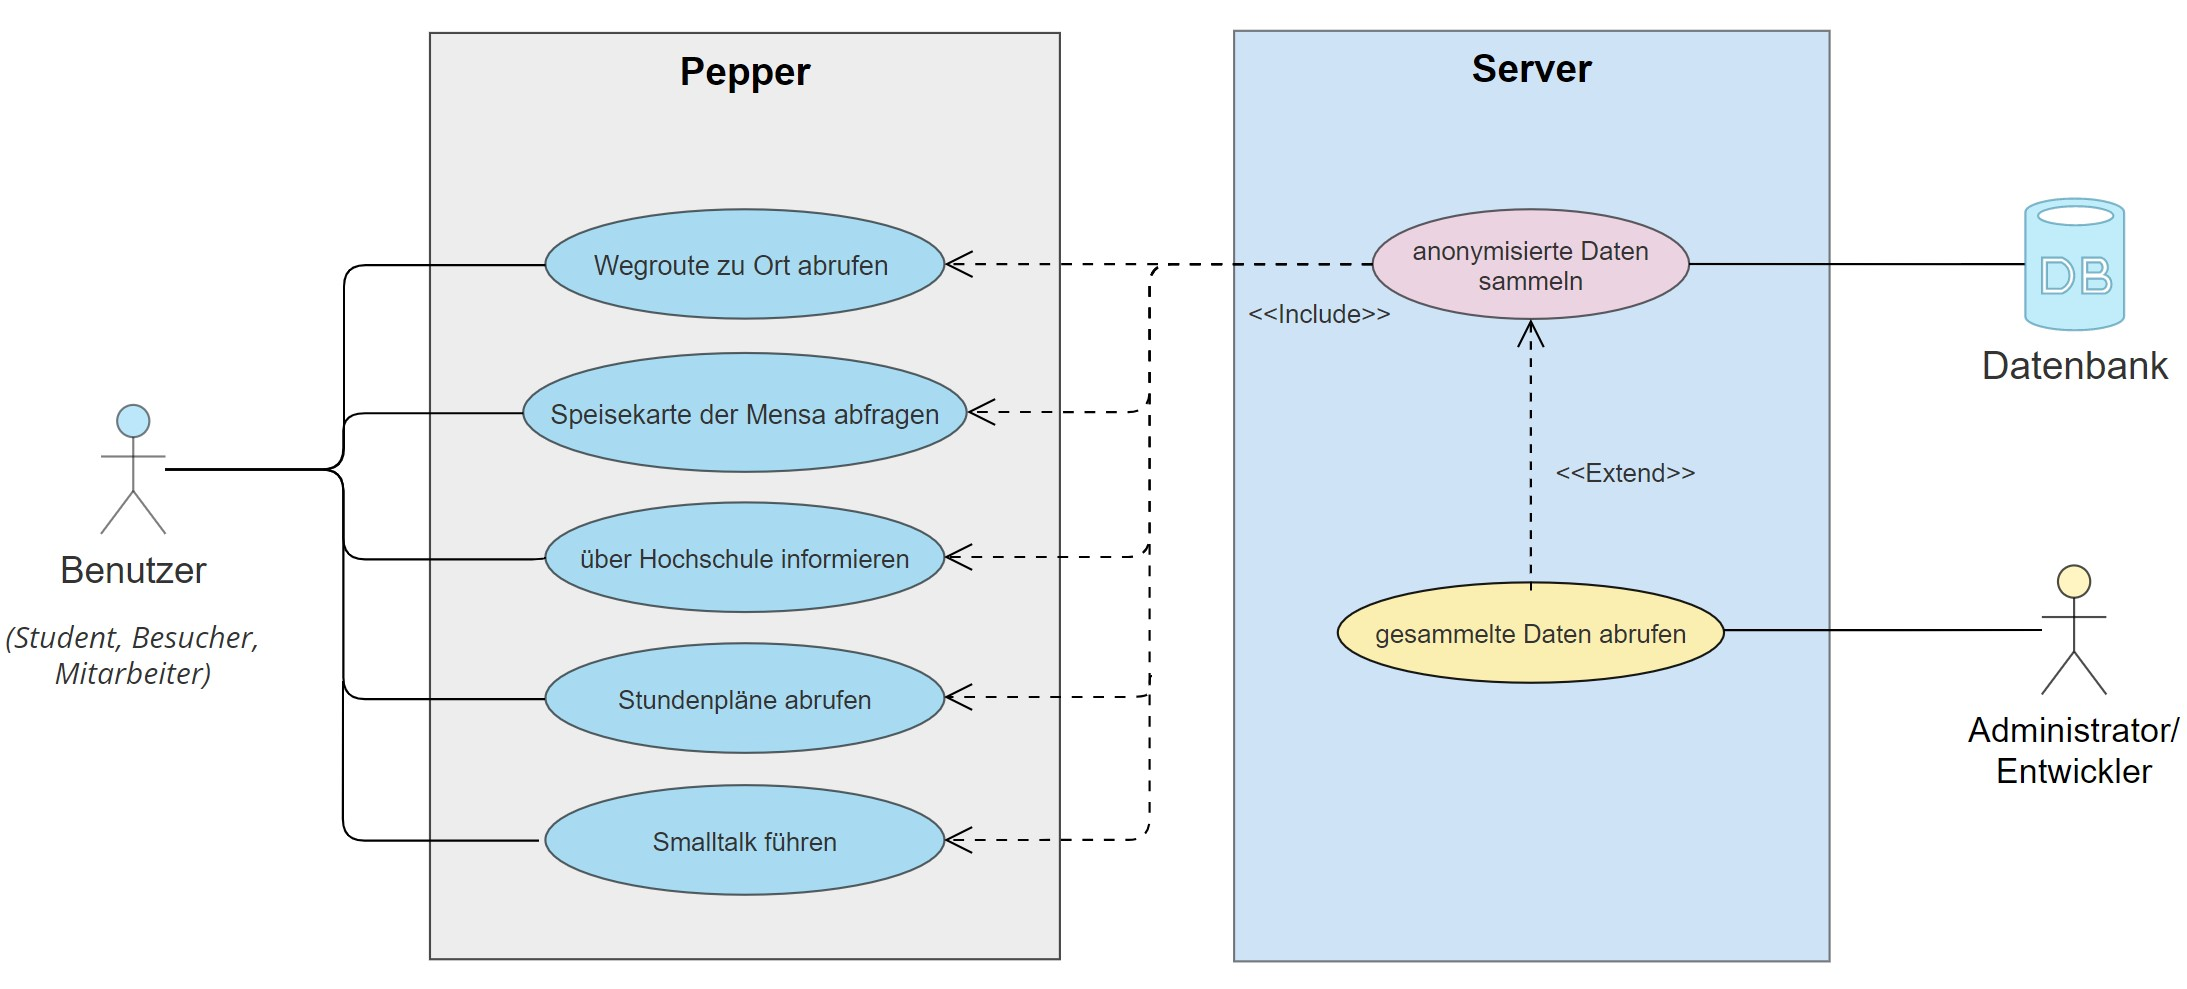
\includegraphics[width=\textwidth]{Figures/use-case-diagram.jpg}
    \caption{Diagramm: Anwendungsfall-Diagramm}
    \label{fig:integration}
    \centering
\end{figure}

Wir haben hierbei die nutzbaren Funktionalitäten für die jeweiligen Akteure der Software voneinander getrennt und in Beziehung zueinander gesetzt. Die Anwendung haben wir in zwei verschiedene Grundsysteme voneinander getrennt. Pepper selbst bietet Funktionalitäten für die Akteure der linken Seite des Diagramms, dies können Studenten, Mitarbeiter, Dozenten oder Besucher der Hochschule sein. Rechts sind die serverseitigen Funktionalitäten der Anwendung darstellt, welche Beispielsweise durch uns Entwickler selbst oder einem zugeteiltem Admin des Systems zur verwendbar sind. Es wäre an dieser Stelle auch denkbar, dass hier an den Daten interessierte Personen der Hochschule, wie beispielsweise Werbeagenturen usw. Zugriff auch diese Funktionalitäten erhalten.

Zudem soll die Interaktion mit Pepper für alle möglich sein. Studierende und Lehrende sollen erfragen können,
wo welche Vorlesung stattfindet, in der Kaffeteria oder Mensa soll sich Pepper mit Gästen unterhalten, Smalltalk führen oder
Empfehlungen für bestimmte Speisen ausgeben. Darüber hinaus wollen wir Pepper das lückenlose Interagieren beibringen, damit er an
besonderen Veranstaltungen, wie dem Tag der offenen Tür oder dem Tag der Informatik, Besuchern Informationen über die Hochschule,
das Leben auf dem Campus, sowie allgemeine Empfehlungen für die Stadt Bremerhaven ausgeben kann.

Die geplante Struktur der Anwendung lässt sich mit der unten dargestellten Abbildung möglichst einfach verdeutlichen.\\

\begin{figure}[H]
    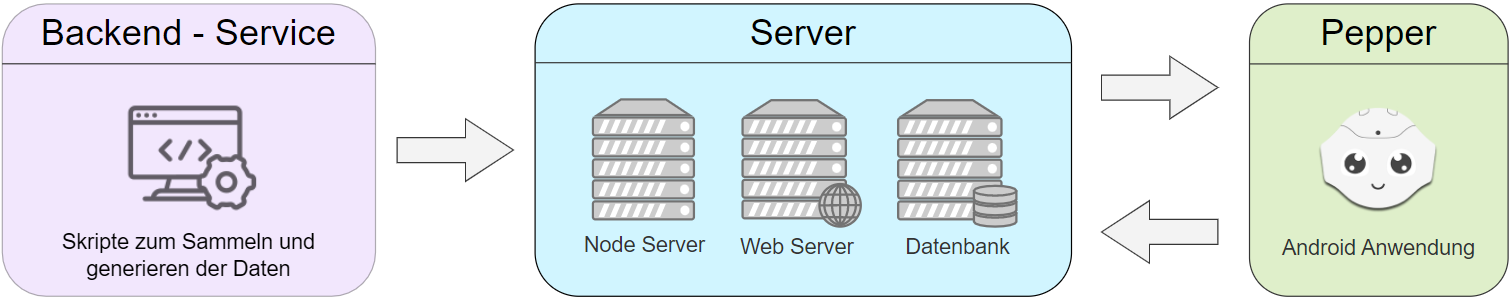
\includegraphics[width=\textwidth]{Figures/anwendungarchitektur.png}
    \caption{Diagramm: Architektur der Anwendung}
    \label{fig:integration}
    \centering
\end{figure}

Die Architektur ist in drei verschiedene Systeme unterteilt, welche in der mit den Pfeilen dargestellten Beziehung zueinander stehen. Hierbei ist der Bereich des Backend-Service ausschließlich dafür da, Daten zu sammeln oder zu generieren, welche dann an den Server gesendet werden. Der Server besteht im groben aus dem Node Server, dem Web Server sowie der Datenbank. Im Gegensatz zu dem Backend-Service steht Pepper mit Server stehen ständig in einem asynchronen Austausch miteinander.\\

\section{Entwicklungsumgebungen für Pepper}

Um das Verhalten von Pepper zu programmieren, kann entweder die Entwicklungsumgebung Android Studio oder Choregraphe verwendet werden. Im Folgenden werden wir auf die einzelnen Softwares eingehen und erklären, wieso wir uns für Android Studio entschieden haben. Anschließend gehen wir noch auf eine weitere Entwicklungsumgebung ein, die aber nicht mehr von Softbanks unterstützt wird.\\

\subsection{Choregraphe}

Mit der Choregraphe Entwicklungsumgebung können komplexe Verhaltensmuster in Pepper integriert werden, ohne eine Zeile Code zu schreiben. Zusätzlich kann das Verhalten aber auch mit der Programmiersprache Python gesteuert werden. Der Choregraphe besitzt mehrer Editoren, mit denen sich zum Beispiel Animationen erstellen lassen können oder Gesprächsfunktionen einbinden lassen. Die Software besitzt ebenfalls einen Emulator mit einem virtuellen Roboter, wo die Applikation getestet werden kann (mehr online: \cite{Choregraphe}).\\

\subsection{Android Studio}

Mit Android Studio können Applikationen für Googles Open-Source Betriebssystem ``Andriod'' entwickelt werden. Sie ist so konzipiert, dass auch Nicht-Programmierer damit arbeiten können, da sie Editoren anbietet, die das Erstellen von Layouts oder Themes vereinfacht. Die Software basiert auf IntelliJ IDEA 14 und bietet die Programmiersprachen Java und Kotlin. Beim Erstellen einer neuen Applikation kann zwischen diesen beiden Programmiersprachen ausgewählt werden.

Die Software besitzt ihren eigenen SDK Manager, worüber die Pepper SDK heruntergeladen werden kann, um eine Entwicklungsumgebung für Pepper zu schaffen. Mit diesen Entwicklungspaketen kommen viele verschiedene Methoden und Funktionen hinzu, worüber sich das Verhalten von Pepper steuern und programmieren lässt. Zusätzlich bietet das Pepper SDK einen Emulator an, wo die Applikation auf einem virtuellen Pepper getestet werden kann und einen weiteren Editor, mit denen Animationen erstellt werden können. Das Tablet von Pepper kann komplett mit den Funktionen und Editoren von Android Studio editiert werden.

Sowohl Android Studio als auch Choregraphe können bestimmte Komponenten von Pepper nicht ansteuern oder verändern. Hierzu gehört zum Beispiel die Kamera von Pepper, da die einzelnen Funktionen wie die Bilderkennung fest verankert sind. Es kann lediglich nur auf die Daten zugegriffen werden, die Pepper selber mit seinen Kameras erzeugt.
(Quelle: \cite{Android_Studio})\\

\subsection{ROS}

Es gab vor beginn unseres Projektes die Möglichkeit, Pepper mit ROS (\textbf{R}obot \textbf{O}perating \textbf{S}ystem) zu entwickeln. ROS ist ein Betriebssystem, das speziell für die Steuerung und Programmierung von Robotern entwickelt wurde. Anders als bei Android Studio oder Choregraphe, besitzt man hier jegliche Freiheiten, den Roboter so zu programmieren, wie man möchte. Zum Beispiel hätten wir mit ROS die Möglichkeit gehabt, auf die Kamera oder Sensoren von Pepper zuzugreifen.
Dies hätte den Vorteil gehabt, dass wir unsere eigene Bild, oder Spracherkennungsalgorithmen für Pepper entwickeln könnten. Softbanks hat sich
jedoch ab einer früheren Version dazu entschieden, die Kompatibilität und Anbindung mit ROS zu stoppen. Hätten wir die Möglichkeit gehabt, ROS zu verwenden, hätten wir uns definitiv dafür entschieden. \\

\section{Entwicklugnsumgebung}

Wir haben uns dazu entschieden, Android Studio als Entwicklungsumgebung zu verwenden, da wir mit der Pepper SDK eine Vielzahl an Möglichkeiten besitzen, Pepper für jede Situation anzupassen. Außerdem wurde es uns auch von den Masterstudenten empfohlen und wir konnten deren Applikation als Referenz verwenden. Für unsere Applikation verwenden wir Java statt Kotlin, da wir in Java schon einige Konzepte in früheren Projekten umgesetzt haben.\\

\section{Hard- und Softwarespezifikationen}
Nachfolgend ist eine Tabelle, welche noch einmal systematisch unsere verwendeten Softwares aufzeigt.
\begin{table}[H]
    \caption{Hard- und Softwarespezifikationen}
    \label{table}
    \setlength{\tabcolsep}{3pt}
    \begin{tabular}{|p{100pt}|p{120pt}|p{180pt}|}
        \hline
        Software / Tool & Version / Spezifikation     & Beschreibung                                                                     \\
        \hline\hline
        Android Studio  & Arctic Fox 2020.3.1 Patch 4 & IDE der IntelliJ Plattform                                                       \\
        \hline
        Gradle          & 7.0.3                       & Build Tool                                                                       \\
        \hline
        Android SDK     & 12                          & Android Framework                                                                \\
        \hline
        Pepper API      & v1.9  API 23                & Entwicklungstools für Pepper mit Emulator, Deploy und Debug Funktion             \\
        \hline
        Android API SDK & 31                          & Framework zum Verbinden und Installieren von Software auf Geräten mit Android OS \\
        \hline
        Java SDK        & 1.8                         & Basis der Programmiersprache Java und dessen Grundfunktionalitäten               \\
        \hline
        \multicolumn{3}{p{380pt}}{Mit abwichenden Versionen kann es zu Kompatibilitätsproblemen kommen.}
    \end{tabular}
    \label{tab1}
\end{table}

% Der Roboter Pepper selbst, ist XXX groß, wurde am XXX von XXX gekauft und ist seit XXX im Besitz der Hochschule
% und läuft derzeit mit der Version XXX.